\documentclass[journal,lettersize]{IEEEtran}

% --- Packages ----------------------------------------------------------------
\usepackage[utf8]{inputenc}
\usepackage[T1]{fontenc}
\usepackage{amsmath,amssymb,amsfonts}
\usepackage{graphicx}
\usepackage{booktabs}
\usepackage{siunitx}
\usepackage{enumitem}
\usepackage{cite}
\usepackage{hyperref}
\usepackage[capitalize]{cleveref}

\hypersetup{colorlinks=true,linkcolor=blue,citecolor=blue,urlcolor=blue}

% \doi{} is used throughout the bibliography but no package defines it;
% this was a pre-existing bug that blocked compilation entirely.
\providecommand{\doi}[1]{\href{https://doi.org/#1}{doi:#1}}

% --- Title Block ---------------------------------------------------------------
\title{Global Fundamental-Parameter Mapping of Lunar Elemental Abundances from Chandrayaan-2 CLASS XRF Data with Cross-Modal Super-Resolution}

\author{Smarak~Kanjilal, Subarno~Maji, \emph{and} Paidi~Geetesh~Chandra% <-this % stops a space
\thanks{All authors are Independent Researchers (e-mail: smarakkanjilal@gmail.com; subarnomaji@kgpian.iitkgp.ac.in; paidigeeteshchandra@gmail.com). ORCID: 0009-0005-4361-3119 (S. Kanjilal); 0009-0006-4698-6882 (S. Maji); 0009-0008-1153-3079 (P. G. Chandra).}% <-this % stops a space
\thanks{\textit{Smarak Kanjilal, Subarno Maji, and Paidi Geetesh Chandra contributed equally to this work.} (Corresponding author: Paidi Geetesh Chandra.)}}

% ==============================================================================
\begin{document}
\maketitle

\begin{abstract}
Mapping the elemental composition of the Moon at high spatial resolution is critical for understanding its geological evolution and resource potential. We present a complete pipeline for lunar elemental abundance mapping from Chandrayaan-2 Large Area Soft X-ray Spectrometer (CLASS) X-ray fluorescence (XRF) data. Raw Level-1 spectra are preprocessed with empirical nightside-background subtraction and a stationary-wavelet-transform plus Savitzky--Golay denoiser, then fitted with a physics-based fundamental-parameter (FP) forward model -- including primary and secondary fluorescence -- using whole-spectrum Trust-Region-Reflective (TRF) optimisation, rather than region-of-interest line-ratio sums. Per-footprint element/Si ratios are projected onto a global $\sim0.33^{\circ}$ grid by centre-point binning with Gaussian smoothing and gap infill. Applied to 1{,}056{,}619 dayside spectra from 24 monthly archives (December~2020--May~2026), the pipeline attains 99.0\% surface coverage at $1^{\circ}$ resolution. We further introduce a cross-modal, optical-guided super-resolution stage that couples the XRF maps to a co-registered optical mosaic through ridge-regularised regression and frequency-domain fusion. On the reliable equatorial-to-mid-latitude band the two clearest tracers behave as expected geologically: Al/Si is the most robust positive correlate of surface brightness ($\rho=+0.43$, bright feldspathic highlands) and Mg/Si the most robust negative correlate ($\rho=-0.39$, dark mafic maria) -- moderate correlations, but the most consistently signed among the six mapped elements. Validation in element/Si ratio space against nine Apollo and Luna landing sites shows the fitted Al/Si ratio tracks ground truth at $r=+0.74$, indicating the pipeline recovers a real compositional signal. Fitted concentrations are reported as relative scale factors pending absolute calibration.
\end{abstract}

\begin{IEEEkeywords}
Lunar remote sensing, X-ray fluorescence spectroscopy, elemental abundance mapping, Chandrayaan-2, fundamental-parameter modeling, cross-modal data fusion, super-resolution.
\end{IEEEkeywords}

% ==============================================================================
\section{Introduction}\label{sec:intro}
\subsection{Background}

\IEEEPARstart{T}{he} composition of the Moon's surface is central to understanding its geological and evolutionary history. Dark basaltic plains mark past volcanism and record the Moon's thermal and magmatic evolution; the surface itself is a mixture of crustal materials, impact-generated deposits, and space-weathering products from solar-wind interaction. Remote sensing has long been used to map global elemental abundances, whose spatial distribution remains central to understanding lunar formation and evolution.

\subsection{Motivation and Objectives}

This study generates high-resolution lunar maps from X-ray fluorescence (XRF) line intensity ratios. Ratioing minimises the influence of external factors such as solar flux and viewing geometry, yielding an independent geochemical view of the surface. The resulting maps characterise compositional heterogeneity relevant to both scientific investigation and in situ resource utilisation, and are intended to contribute toward the next generation of lunar mapping missions.

\subsection{XRF Spectroscopy Overview}
X-ray fluorescence (XRF) spectroscopy is a well-established technique for characterising the Moon's surface composition \cite{Jenkins1999,Beckhoff2006}. The Chandrayaan-1 X-ray Spectrometer (C1XS) provided early geochemical insight into regions such as the southern highlands, validated against laboratory experiments and Monte Carlo simulations. The Chandrayaan-2 Large Area Soft X-ray Spectrometer (CLASS) then improved spatial resolution and sensitivity \cite{Narendranath2020}, with demonstrated spatial resolutions of 150 to 15\,km. Challenges remain from factors affecting XRF line intensities -- incident solar spectrum, matrix effects, particle size, and geometry (angle of incidence, phase angle) -- particularly in nadir-viewing configurations like CLASS.

\subsection{Previous Work}
Several lunar missions have advanced understanding of surface composition through direct sampling and remote sensing. The Lunar Prospector gamma-ray spectrometer (GRS) produced the first global elemental maps \cite{Lawrence1998} at coarse (tens to hundreds of km) resolution, mapping thorium and potassium well but struggling with Mg, Al, and Si owing to moderate spectral resolution and detector background. Chandrayaan-1 and -2 (C1XS, CLASS) subsequently improved spatial resolution and sensitivity for XRF line ratios such as Mg/Si and Al/Si. Lunar soil samples from Apollo, Luna, and Chang'E-5, together with rover-based in situ measurements, provide complementary ground-truth references.

Machine learning has further advanced lunar composition analysis. LSCC reflectance spectra have been classified with Support Vector Machines and penalised logistic regression to determine particle size and maturity \cite{Kodikara2020}. Particle Swarm Optimisation coupled with XGBoost (PSO-XGBoost) has modelled oxide abundances against geochemical indicators to yield high-resolution global oxide maps \cite{Wu2024}, and Bayesian-optimised XGBoost has been applied to landing-site safety assessment, outperforming CNNs and Random Forests on feature importance \cite{Wen2024}. Chang'E-5 data analysed with 1d-CNN models have produced detailed oxide distribution maps \cite{Yang2023}, underscoring the growing role of deep learning in lunar surface analysis; unlike these learned methods, the fundamental-parameter approach adopted here requires no training data, at the cost of the simplifications noted in \cref{sec:secondary,sec:discussion}.



\section{Spectral Preprocessing}\label{sec:preprocessing}

\subsection{Data acquisition}
The X-ray spectral data used in this study were acquired from the Chandrayaan-2 Large Area Soft X-ray Spectrometer (CLASS). The dataset was obtained from the PRADAN (Policy-based Data Retrieval, Analytics, Dissemination, and Notification system) portal hosted by the Indian Space Science Data Centre (ISSDC), Indian Space Research Organisation (ISRO). The data comprise 24 non-contiguous monthly archives spanning December~2020 to May~2026, totalling 1{,}515{,}239 raw Level-1 exposures.

CLASS performs X-ray fluorescence (XRF) spectroscopy using Swept Charge Devices (SCDs) to detect characteristic X-rays from the lunar surface, operating in the soft X-ray band (0.8--15\,keV) to map major rock-forming elements including Mg, Al, Si, Ca, Ti, and Fe. Raw files were accessed in FITS format, containing photon counts, exposure times, and detector gain information.

\subsection{Data Preprocessing}

A custom pipeline processes the raw spectra and extracts elemental fluxes in four stages: reference calibration, background subtraction, signal denoising, and flux integration.

1. Reference Energy Calibration:
Accurate reference energies for the target elements (O, Mg, Al, Si, Ca, Ti, Fe) were established using the xraydb database. The $K$-shell emission lines were queried for each element. Priority was given to the $K_{\alpha1}$ line; however, if unavailable, the generic $K_{\alpha}$ line was selected. These reference energies (in keV) served as the central centroids for the Region of Interest (ROI) calculations.

2. Background Subtraction:
As no dedicated background file ships with this CLASS data release, a reference background spectrum was constructed empirically by averaging the nightside exposures ($\mathrm{SOLARANG} \geq 90^{\circ}$) within each monthly batch, which receive negligible solar-driven fluorescence and so capture the instrumental and cosmic background. Both spectra were normalised by exposure time to count rates (counts/s), the background rate was subtracted, and a non-negativity constraint was applied to the result.

3. Signal Denoising:
To improve the signal-to-noise ratio, a multi-stage denoising approach was utilized. First, a Stationary Wavelet Transform (SWT) was applied to the background-subtracted signal using the Symlet-8 (sym8) wavelet at decomposition level 2 \cite{Mallat2009}. Soft thresholding was applied to the detail coefficients, with the threshold dynamically determined from the signal's noise variance ($\sigma$). Following wavelet reconstruction, the spectrum was smoothed using a Savitzky--Golay filter (window length 7, polynomial order 3) \cite{Savitzky1964} to preserve spectral line shapes while reducing high-frequency noise.

4. Flux Integration:
Unlike traditional ROI-sum XRF analysis, the denoised spectrum is not collapsed into a single integrated count per element here. Instead, the full background-subtracted, denoised, non-negativity-constrained count-rate array is retained across all $N_{\mathrm{ch}}$ channels and passed directly as the measured spectrum $\mathbf{S}_{\mathrm{meas}}$ to the whole-spectrum fundamental-parameter fit (\cref{sec:fitting}). This is necessary because the K$\alpha$/K$\beta$ lines of adjacent light elements (e.g.\ Mg, Al, Si) partially overlap once convolved with the detector response (\cref{sec:gaussian}); a discrete ROI sum would conflate these, whereas the whole-spectrum TRF fit can disentangle them using the full model shape, including secondary-fluorescence cross-terms (\cref{sec:secondary}).

\begin{figure}[!t]
  \centering
  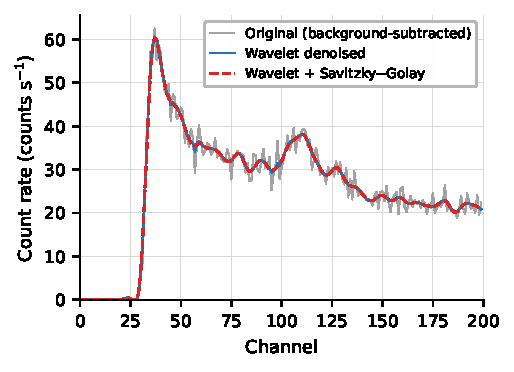
\includegraphics[width=\linewidth]{../outputs/figures/final/fig1_preprocessing.pdf}
  \caption{Spectral preprocessing pipeline (\cref{sec:preprocessing}):
    raw count-rate spectrum, background-subtracted spectrum, and the final
    wavelet+Savitzky--Golay denoised spectrum, overlaid for one
    representative dayside exposure. Dashed vertical lines mark the
    K$\alpha$ line energies of Mg, Al, Si, Ca, Ti, and Fe.}
  \label{fig:preprocessing}
\end{figure}

\Cref{fig:preprocessing} illustrates the three-stage preprocessing
pipeline on one representative dayside exposure.

\section{Fundamental-Parameter Forward Model}\label{sec:fp_model}

Quantitative analysis of XRF spectra can follow either an
\emph{empirical} calibration approach or a \emph{fundamental-parameter}
(FP) approach.  The FP method derives fluorescence intensities directly
from the physics of X-ray interaction with matter, avoiding the need for
matrix-matched calibration standards
\cite{Sherman1955,Shiraiwa1966,Criss1968}.  This section describes the
FP forward model used in the pipeline.

\subsection{Atomic Data and Line Setup}\label{sec:atomic}

\subsubsection{Line Energies and Radiative Rates}

For each element (identified by atomic number $Z$), the model retrieves
K-series emission line energies and radiative rates from the
\texttt{xraylib} database \cite{Schoonjans2011}:
\begin{align}
  E_\ell &: \text{line energy for transition } \ell, \label{eq:line_energy}\\
  p_\ell &: \text{radiative rate for transition } \ell. \label{eq:rad_rate}
\end{align}
The lines included are K$\alpha_1$ and K$\beta_1$.  L-series lines are
supported in the framework but are not employed for the light-to-medium-$Z$
elements considered here.

Lines are grouped by \emph{type} (K$\alpha$, K$\beta$, L$\alpha$,
L$\beta$), and for each type a \emph{mean energy} is computed:
\begin{equation}\label{eq:mean_energy}
  \bar{E}_t = \frac{1}{|\mathcal{L}_t|}
    \sum_{\ell \in \mathcal{L}_t} E_\ell,
\end{equation}
where $\mathcal{L}_t$ is the set of lines belonging to type~$t$.

\subsubsection{Mass Attenuation Coefficient}

The total mass attenuation coefficient $\mu(E)$ [\si{cm^2/g}] at a
given energy $E$ is obtained from tabulated cross-sections:
\begin{equation}\label{eq:cs_total}
  \mu_i(E) = \sigma_{\mathrm{total}}(Z_i, E),
\end{equation}
which includes photoelectric, coherent (Rayleigh), and incoherent
(Compton) contributions.  This quantity is used both for primary
intensity calculations and for secondary fluorescence cross-terms.

\subsubsection{Jump Factor}\label{sec:jump_factor}

At an absorption edge of shell~$s$, the mass attenuation coefficient
exhibits a discontinuity characterised by the \emph{jump ratio}~$r_s$.
The \emph{jump factor} is defined as:
\begin{equation}\label{eq:jump_factor}
  \boxed{J_s = 1 - \frac{1}{r_s}}
\end{equation}
The jump factor represents the fraction of total photoelectric
absorption attributable to shell~$s$ ionisation.  Just below the K-edge,
only L, M, \ldots\ shells contribute; at the edge, K-shell ionisation
becomes energetically accessible, causing a discontinuous increase in
the cross-section.

\subsubsection{Fluorescence Yield}

The fluorescence yield~$\omega_s$ is the probability that a vacancy in
shell~$s$ is filled radiatively (X-ray emission) rather than by Auger
emission.  For the elements in the model, $\omega$ increases with atomic
number (e.g.\ $\omega_\mathrm{K}(\mathrm{Mg}) \approx 0.02$,
$\omega_\mathrm{K}(\mathrm{Fe}) \approx 0.33$).

\subsubsection{Elemental Constant}\label{sec:elem_const}

Combining the three fundamental quantities above, the \emph{elemental
constant} for element~$i$ at emission line~$\ell$ (belonging to
shell~$s$) is:
\begin{equation}\label{eq:elemental_const}
  \boxed{K_{i,\ell} = J_s^{(i)} \cdot \omega_s^{(i)} \cdot p_\ell^{(i)}}
\end{equation}
The shell is determined from the line type: K$\alpha$ or K$\beta$ lines
correspond to the K shell ($s=0$), while L$\alpha$ or L$\beta$ lines
correspond to the L shell ($s=1$).

\subsection{Primary Fluorescence Intensity}\label{sec:primary}

The primary fluorescence intensity for element~$i$ at emission
line~$\ell$ is proportional to its mass attenuation coefficient
evaluated at the emission line energy:
\begin{equation}\label{eq:primary}
  \boxed{I_{i,\ell}^{(\mathrm{P})} = \mu_i(E_\ell)}
\end{equation}

\subsection{Secondary Fluorescence Intensity}\label{sec:secondary}

Secondary fluorescence occurs when a characteristic photon emitted by
element~$j$ is absorbed by element~$i$, causing additional fluorescence
of element~$i$.  This inter-element enhancement effect is particularly
important in multi-element lunar samples where the mutual excitation
between neighbouring elements can significantly alter the observed
intensities.

The secondary intensity contribution to line~$\ell$ of
element~$i$ (the analyte) is:
\begin{equation}\label{eq:secondary}
  \boxed{
    I_{i,\ell}^{(\mathrm{S})} =
      \sum_{\substack{j=1\\j\neq i}}^{N}\;\sum_{m \in \mathcal{L}_j}
        \mu_j(E_m) \cdot \mu_i(E_m) \cdot K_{i,\ell} \cdot \beta_{j,m}
  }
\end{equation}
where:
\begin{itemize}[nosep]
  \item $\mu_j(E_m)$: mass attenuation coefficient of element~$j$ at the
        energy of its own emission line~$m$.
  \item $\mu_i(E_m)$: mass attenuation coefficient of element~$i$ (the
        analyte) at the energy of element~$j$'s emission line~$m$,
        quantifying how strongly $i$ absorbs $j$'s fluorescence.
  \item $K_{i,\ell}$: the elemental constant for the analyte line
        (\cref{eq:elemental_const}).
  \item $\beta_{j,m} \in [0,\infty)$: an adjustable enhancement factor
        for element~$j$, line~$m$ (default value~1.0), accounting for
        geometry-dependent effects not captured by the simplified
        formula.
\end{itemize}

The outer sum runs over all elements $j \neq i$; the inner sum runs over
all available emission lines~$m$ of element~$j$. For simplicity, the
geometric terms ($\psi$, $\phi$) of the full Sherman~(1955) secondary-
fluorescence formulation are absorbed into the scale factor~$s$
(\cref{eq:spectrum}), which is fitted per spectrum.

\subsection{Total Fluorescence Intensity}\label{sec:total}

The total fluorescence intensity for element~$i$ at line~$\ell$,
combining primary and secondary excitation, is:
\begin{equation}\label{eq:total_intensity}
  \boxed{
    I_{i,\ell}^{(\mathrm{tot})} = C_i \cdot \bigl[
      I_{i,\ell}^{(\mathrm{P})} + I_{i,\ell}^{(\mathrm{S})}
    \bigr]
  }
\end{equation}
where $C_i$ is the concentration (weight fraction) of element~$i$.
The emitted intensity is thus proportional to both the analyte abundance
and the strength of the excitation channels.

\subsection{Gaussian Detector Response}\label{sec:gaussian}

An energy-dispersive detector has finite energy resolution that broadens
each monochromatic emission line into a peak with an approximately
Gaussian profile.  The detector-response function for a line at
energy~$E_\ell$ is:
\begin{equation}\label{eq:gaussian}
  \boxed{
    G(E;\,E_\ell,\,\sigma) =
      \frac{1}{\sigma\sqrt{2\pi}}\,
      \exp\!\left[-\frac{(E - E_\ell)^2}{2\sigma^2}\right]
  }
\end{equation}
where $\sigma$ is the standard deviation, related to the full width at
half maximum (FWHM) by:
\begin{equation}\label{eq:fwhm}
  \mathrm{FWHM} = 2\sqrt{2\ln 2}\;\sigma \approx 2.355\,\sigma.
\end{equation}

\subsection{Synthetic Spectrum Assembly}\label{sec:spectrum}

\subsubsection{Channel Discretisation}

The energy axis is discretised into detector channels:
\begin{equation}\label{eq:channel_energy}
  E_k = k \cdot \Delta E, \qquad k = 0, 1, \dots, N_{\mathrm{ch}}-1,
\end{equation}
where $N_{\mathrm{ch}}$ is the number of channels and $\Delta E$ is the
energy per channel:
\begin{equation}\label{eq:energy_factor}
  \Delta E =
  \begin{cases}
    0.0135~\text{keV/channel} & \text{for } N_{\mathrm{ch}} = 2048,\\[3pt]
    0.0277~\text{keV/channel} & \text{for } N_{\mathrm{ch}} = 1024.
  \end{cases}
\end{equation}

\subsubsection{Windowed Gaussian Convolution}

For each element~$i$ and each line~$\ell$, the Gaussian convolution is
evaluated only within a truncation window of $\pm\sigma$ around the line
centre~$\bar{E}_t$ (the mean energy of the line type).  The bin
boundaries are:
\begin{align}
  k_{\mathrm{start}} &= \max\!\left(0,\;
    \left\lfloor\frac{\bar{E}_t - \sigma}{\Delta E}
    \right\rfloor\right), \label{eq:binstart}\\
  k_{\mathrm{end}} &= \min\!\left(N_{\mathrm{ch}},\;
    \left\lfloor\frac{\bar{E}_t + \sigma}{\Delta E}
    \right\rfloor\right). \label{eq:binend}
\end{align}

The number of evaluation points within the window is:
\begin{equation}\label{eq:num_bins}
  N_{\mathrm{bins}} = \left\lfloor
    \frac{2\sigma}{\Delta E}
  \right\rfloor + 1.
\end{equation}

\subsubsection{Full Spectrum Formula}

The total synthetic spectrum is the sum over all elements and all their
lines:
\begin{equation}\label{eq:spectrum}
  \boxed{
    \begin{aligned}
      S_{\mathrm{model}}(E_k) &= s \sum_{i=1}^{N}\;\sum_{\ell \in \mathcal{L}_i}
        I_{i,\ell}^{(\mathrm{tot})} \cdot G(E_k;\,\bar{E}_t,\,\sigma) \\
      &\quad\text{for } k \in [k_{\mathrm{start}},\,k_{\mathrm{end}})
    \end{aligned}
  }
\end{equation}
where $s$ is a global scale factor and $\bar{E}_t$ is the mean energy
of the line type containing~$\ell$.

% ==============================================================================
\section{Spectral Fitting Procedure}\label{sec:fitting}

The forward model described in \cref{sec:fp_model} is fitted to each
measured spectrum to determine the elemental concentrations and
instrument parameters.  The nine free parameters to be determined are:
\begin{equation}\label{eq:params}
  \boldsymbol{\theta} = \bigl(
    C_{\mathrm{Fe}},\, C_{\mathrm{Al}},\, C_{\mathrm{Mg}},\,
    C_{\mathrm{Si}},\, C_{\mathrm{Ca}},\, C_{\mathrm{Ti}},\,
    C_{\mathrm{O}},\; s,\; \sigma
  \bigr) \in \mathbb{R}^{9},
\end{equation}
comprising the weight-fraction concentrations of seven elements, a
global scale factor~$s$, and the detector resolution
parameter~$\sigma$.

The fit solves the following bound-constrained least-squares problem:
\begin{equation}\label{eq:objective}
  \min_{\boldsymbol{\theta}}\;
    \bigl\|\mathbf{S}_{\mathrm{meas}}
      - \mathbf{S}_{\mathrm{model}}(\boldsymbol{\theta})\bigr\|_2^2
  \quad\text{subject to}\quad
  \boldsymbol{\theta}_{\min} \leq \boldsymbol{\theta}
    \leq \boldsymbol{\theta}_{\max},
\end{equation}
where the element-wise bounds
$\boldsymbol{\theta}_{\min}$ and $\boldsymbol{\theta}_{\max}$ are given
in \cref{tab:bounds}, and the residual vector is
$\mathbf{r}(\boldsymbol{\theta}) =
  \mathbf{S}_{\mathrm{meas}} -
  \mathbf{S}_{\mathrm{model}}(\boldsymbol{\theta})$.

\begin{table}[!t]
  \centering
  \caption{Bound constraints used in the TRF fit for each parameter in
    $\boldsymbol{\theta}$ (\cref{eq:params}). The concentration bound of
    200 is not a wt\% limit: $C_i$ are unitless relative scale factors,
    not calibrated to wt\% (\cref{sec:units_caveat}).}
  \label{tab:bounds}
  \begin{tabular}{lcc}
    \toprule
    \textbf{Parameter} & $\theta_{\min}$ & $\theta_{\max}$ \\
    \midrule
    $C_{\mathrm{Fe}},\,C_{\mathrm{Al}},\,C_{\mathrm{Mg}},\,C_{\mathrm{Si}},\,C_{\mathrm{Ca}},\,C_{\mathrm{Ti}},\,C_{\mathrm{O}}$ & 0 & 200 \\
    $s$ (scale) & $10^{-8}$ & 1 \\
    $\sigma$ (keV) & 0.01 & 0.5 \\
    \bottomrule
  \end{tabular}
\end{table}

At each optimiser iteration, the forward model extracts the current
concentrations, scale, and resolution from the parameter vector;
computes the primary and secondary fluorescence intensities for every
element and emission line; convolves each line contribution with the
Gaussian detector-response function within the appropriate windowed
channel range; and sums all contributions scaled by~$s$ to produce the
synthetic spectrum $S_{\mathrm{model}}(\boldsymbol{\theta})$.

The minimisation employs the Trust-Region Reflective (TRF) algorithm
\cite{Branch1999}, which is well-suited for bound-constrained nonlinear
least-squares problems.  The TRF method iteratively constructs a local
quadratic model of the objective function within a trust region, solving
a sequence of constrained sub-problems to converge on the optimal
parameter vector $\boldsymbol{\theta}^*$.  The pipeline is designed for
batch processing of large spectral datasets: each spectrum from the
catalogue is a 1D array of photon counts with
$N_{\mathrm{ch}} = 2048$ channels, and multiple spectra are
processed in parallel to handle the large volume of CLASS observations
efficiently.

\subsection{Units Caveat}\label{sec:units_caveat}

The concentration parameters $C_i$ recovered by the fit (\cref{eq:params})
are relative scale factors internally consistent with the
primary/secondary fluorescence formulation of \cref{sec:fp_model}, not
concentrations calibrated to weight percent (wt\%): no matrix-matched
standards or absolute-intensity calibration were used. $C_i$ values
throughout this paper (\cref{tab:regression,tab:correlation,tab:ablation}
and \cref{sec:mapping,sec:superres}) should therefore be read as
internally consistent relative abundances, informative for spatial
pattern and element-to-element ratios but not calibrated wt\% figures. A
one-point or linear calibration against a reference dataset (e.g.\
Apollo geochemistry, \cref{sec:validation}) is a necessary next step
before absolute wt\% maps can be produced; \cref{sec:validation}
validates in ratio space (element/Si) for exactly this reason.

\begin{figure}[!t]
  \centering
  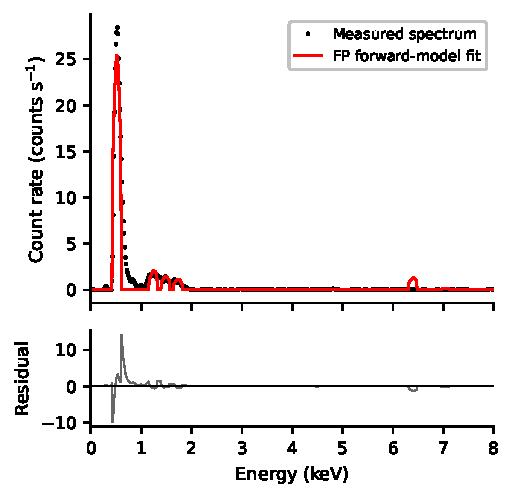
\includegraphics[width=\linewidth]{../outputs/figures/final/fig2_fitted_spectrum.pdf}
  \caption{A representative measured spectrum (black dots) with its
    best-fit fundamental-parameter model (red line) and fit residuals
    (bottom panel), zoomed to $0$--$8$\,keV where all modeled line energies
    lie. The spectrum shown was selected as the one closest to the median
    TRF cost among the top-flux quartile of successfully fitted spectra
    (i.e.\ the higher-signal population the maps and super-resolution
    stage are actually built from, \cref{sec:mapping}), so the line
    structure -- rather than a near-featureless low-count exposure -- is
    visible. Converged concentrations for this spectrum: Fe~0.00484,
    Al~0.04714, Mg~0.08601, Si~0.02846, Ca~0.00009, Ti~0.00008, O~13.586
    (relative units, \cref{sec:units_caveat}); O's value is orders of
    magnitude larger because its soft, poorly-resolved K$\alpha$ line
    (0.52\,keV) causes its parameter to absorb low-energy continuum
    rather than track a resolved line, so it is not used as a
    quantitative abundance anywhere in this paper. Scale
    $s=2.64\times10^{-5}$, $\sigma=0.083$~keV, cost~441.5.}
  \label{fig:fitted_spectrum}
\end{figure}

\section{Spatial Abundance Mapping}\label{sec:mapping}

Once elemental concentrations have been determined for each spectrum, the
fitted values are projected onto a geographic grid to produce spatial
abundance maps.

\subsection{Ratio Quantity and Outlier Handling}\label{sec:map_ratio}

Rather than mapping the raw fitted concentration $C_i$, we map the
\emph{element/silicon ratio} $C_i / C_{\mathrm{Si}}$. Because each fit's
overall amplitude is absorbed into the per-spectrum scale factor~$s$
(\cref{sec:units_caveat}), which varies with solar flux and viewing
geometry from exposure to exposure, ratioing to a common denominator
(Si, a ubiquitous major element) cancels that nuisance amplitude and
yields a quantity that reflects surface composition far more faithfully --
the standard practice for lunar XRF line-ratio mapping (e.g.\ Mg/Si,
Al/Si). Before mapping, the per-footprint ratio distribution is cleaned
in two steps: a $\log(1+x)$ transform followed by a $1.5\times$
interquartile-range cut removes extreme outliers (a handful of near-zero
$C_{\mathrm{Si}}$ fits produce non-physical ratios), and a high-percentile
cap trims the residual upper tail so the colour scale reflects the bulk of
the distribution.

\subsection{Rasterisation and Smoothing}\label{sec:map_raster}

Each observation carries a quadrilateral footprint with vertices
$(\mathrm{lat}_k, \mathrm{lon}_k)$, $k=0,\dots,3$. The footprint is
reduced to its geometric centre $(\bar{\mathrm{lat}}, \bar{\mathrm{lon}})$
and binned onto an equirectangular grid of width $N$ and height $N/2$
(default $N=1080$, i.e.\ $\sim0.33^{\circ}$ per pixel) at indices
\begin{equation}\label{eq:bin_index}
  j = \left\lfloor \frac{\bar{\mathrm{lon}}+180}{360}\,N \right\rfloor,
  \qquad
  i = \left\lfloor \frac{\bar{\mathrm{lat}}+90}{180}\,\frac{N}{2} \right\rfloor .
\end{equation}
Each cell accumulates the sum of contributing ratio values and a count;
their quotient gives the per-cell mean. To suppress per-pixel sampling
noise while preserving structure, both the summed-value grid and the
occupancy mask are convolved with a Gaussian ($\sigma=1.1$ px) and the
smoothed value is renormalised by the smoothed occupancy:
\begin{equation}\label{eq:smooth_renorm}
  \tilde{\mathbf{A}}(x,y) =
  \frac{\bigl(G_\sigma * \mathbf{V}\bigr)(x,y)}
       {\bigl(G_\sigma * \mathbf{W}\bigr)(x,y)},
\end{equation}
where $\mathbf{V}$ is the per-cell mean grid (zero-filled) and
$\mathbf{W}$ is the binary occupancy. Interior gaps between adjacent
orbital tracks are then filled by replacing each still-empty cell with the
mean of its populated $3\times3$ neighbours. The spatial coverage is
reported as the fraction of grid cells directly populated before infill.
For the cross-modal correlation and super-resolution analysis
(\cref{sec:superres}) the maps are additionally restricted to
$|\phi|<60^{\circ}$, excluding the high-latitude bins where the grazing
solar-incidence geometry of a nadir-viewing instrument makes the retrieved
ratios least reliable.



\section{Cross-Modal Guided Super-Resolution of Elemental Abundance Maps}%
\label{sec:superres}

The elemental abundance maps produced by the spatial mapping stage
(\cref{sec:mapping}) are inherently limited in spatial resolution by the
CLASS instrument footprint ($r_a \approx \SI{12}{km/pixel}$).  We
formulate the resolution enhancement as a \emph{cross-modal guided
super-resolution} problem \cite{Ham2018}: a high-resolution guide
image from one modality (optical reflectance) is used to inject spatial
detail into a co-registered low-resolution target from a different
modality (XRF-derived elemental abundance).  Unlike classical
single-image super-resolution, the guide signal provides physically
grounded structural priors---surface reflectance patterns encode
compositional boundaries---enabling reconstruction well beyond the
Nyquist limit of the XRF sensor alone.  The approach is related to
pan-sharpening \cite{Vivone2015}, but differs in that the guide and
target originate from fundamentally different sensing physics (optical
vs.\ X-ray fluorescence), making it a true cross-modal data fusion
task.

Let $\mathbf{I} \in \mathbb{R}^{H_o \times W_o}$ denote the
high-resolution optical image of the lunar surface acquired at spatial
resolution $r_o = \SI{0.4}{km/pixel}$, and let
$\mathbf{A} \in \mathbb{R}^{H_a \times W_a}$ denote the low-resolution
elemental abundance map at resolution $r_a = \SI{12}{km/pixel}$.
Because $r_a \gg r_o$, the abundance map lacks the spatial sharpness
necessary for detailed geological analysis; however, the optical image
encodes surface reflectance variations that are inherently linked to
compositional differences, since different elements interact uniquely
with incident solar radiation.

The enhancement proceeds in four steps: (i)~spatial alignment of the
two data sources, (ii)~learning a pixel-wise intensity-to-abundance
transformation, (iii)~frequency-domain extraction of fine spatial
detail, and (iv)~fusion of the transformed and smoothed components into
the final enhanced map.

\paragraph{Spatial alignment.}
The optical image is first downscaled to a target resolution
$r_t = \SI{1.2}{km/pixel}$ via structured resampling, yielding the
reduced image
\begin{equation}\label{eq:downscale}
  \mathbf{I}_{\downarrow} = \mathcal{R}_{r_o \to r_t}(\mathbf{I})
  \;\in\; \mathbb{R}^{H_t \times W_t},
\end{equation}
where $\mathcal{R}$ denotes the resampling operator designed to minimise
aliasing artefacts while preserving essential geological structure.  The
abundance map is then interpolated to the same dimensions using
nearest-neighbour interpolation:
\begin{equation}\label{eq:interp}
  \hat{\mathbf{A}} = \mathcal{N}_{r_a \to r_t}(\mathbf{A})
  \;\in\; \mathbb{R}^{H_t \times W_t}.
\end{equation}
Nearest-neighbour interpolation preserves the original abundance values
and avoids introducing artificial gradients, although it produces
blocky artefacts that are addressed in the subsequent fusion stage.

\subsection{Intensity--Abundance Correlation}\label{sec:sr_correlation}

With the two images co-registered at resolution~$r_t$, the pixel-wise
correlation between optical intensity and elemental abundance is
quantified via Pearson's coefficient:
\begin{equation}\label{eq:pearson}
  \rho = \frac{
    \sum_{i}\bigl(\mathbf{I}_{\downarrow,i} - \bar{\mathbf{I}}_\downarrow\bigr)
    \bigl(\hat{\mathbf{A}}_i - \bar{\hat{\mathbf{A}}}\bigr)
  }{
    \sqrt{\sum_{i}\bigl(\mathbf{I}_{\downarrow,i}
      - \bar{\mathbf{I}}_\downarrow\bigr)^2}\;
    \sqrt{\sum_{i}\bigl(\hat{\mathbf{A}}_i
      - \bar{\hat{\mathbf{A}}}\bigr)^2}
  },
\end{equation}
where the sums run over all co-located pixels~$i$.  The coefficients
were computed from the element/Si ratio maps (\cref{sec:mapping}) built
from the 855{,}190 TRF-fitted spectra (\cref{sec:results_fitting}) and
compared with the optical guide (\cref{tab:correlation}). Mapping the
element/Si \emph{ratio} rather than the raw relative concentration is
essential here: the ratio cancels the per-spectrum scale factor (which
absorbs solar-flux and geometry variations), leaving a quantity that
tracks true surface composition far more cleanly. The comparison is
further restricted to the equatorial-to-mid-latitude band
$|\phi| < 60^{\circ}$, where the nadir-viewing geometry is most reliable.
Aluminium is the most robustly, positively correlated element with
surface brightness ($\rho = +0.43$), exactly as expected from the
bright, Al-rich anorthositic highlands \cite{Lucey2000}, and it is
adopted as the headline element for cross-modal guided super-resolution.
Magnesium is the most robustly negative ($\rho = -0.39$), consistent
with the optically dark, mafic-rich basaltic maria. Both are moderate
correlations ($R^2\approx0.16$--$0.19$), not strong ones, but the
largest-magnitude and most consistently signed among the six mapped
elements. The remaining elements correlate only weakly with albedo
(\cref{tab:correlation}); Al and Mg are thus the two clearest optical
tracers, of the feldspathic highlands and the mafic maria respectively.

\begin{table}[!t]
  \centering
  \caption{Pearson correlation coefficients between optical intensity
    and element/Si abundance ratio, computed from the 855{,}190 fitted
    spectra on the $|\phi|<60^{\circ}$ reliable band (see text). Aluminium
    (highlands) and magnesium (mafic maria) are the two largest-magnitude,
    oppositely-signed tracers (moderate correlations, $R^2\approx0.16$--$0.19$;
    \cref{sec:sr_correlation}).}
  \label{tab:correlation}
  \begin{tabular}{lc}
    \toprule
    \textbf{Element} & \textbf{Pearson Correlation ($\rho$)} \\
    \midrule
    Al   &  $+0.429$ \\
    Mg   &  $-0.394$ \\
    O    &  $+0.158$ \\
    Fe   &  $+0.104$ \\
    Ca   &  $+0.020$ \\
    Ti   &  $+0.012$ \\
    \bottomrule
  \end{tabular}
\end{table}

\subsubsection{Reproducibility and Sample-Size Caveats}\label{sec:sr_correlation_caveat}

The headline Al/Si correlation is far stronger and more stable than the
earlier, small-dataset numbers, owing to the ratio normalisation,
near-global coverage (\cref{sec:results_coverage}), and the latitude
restriction. Progressively excluding the poles moves it from $\rho=+0.23$
(full sphere) to $+0.36$/$+0.43$/$+0.52$ at $|\phi|<70^{\circ}/60^{\circ}/50^{\circ}$
-- monotonic and correctly signed, unlike the sign-flipping seen on
raw-concentration maps. The $|\phi|<60^{\circ}$ band retains $\sim$67\%
of the surface and over a quarter-million co-located pixels per element.
These pixels are not statistically independent: the Gaussian
smoothing of \cref{sec:map_raster} ($\sigma=1.1$\,px) correlates
adjacent cells by construction, so the nominal pixel count overstates the
effective degrees of freedom and a raw-$N$ significance level would be
optimistic. We therefore treat $\rho$'s magnitude and sign stability
above, not raw-$N$ significance, as the relevant evidence, and weight the
independent, footprint-level Apollo/Luna validation
(\cref{sec:validation}) accordingly.

\subsection{Intensity-to-Abundance Regression}\label{sec:sr_regression}

The correlations above motivate a transformation function
$F_d : \mathbb{R} \to \mathbb{R}$ that maps optical intensity to
elemental abundance.  A ridge-regularised polynomial regression of
degree~$d$ is fitted independently for each element:
\begin{equation}\label{eq:poly_regression}
  \begin{aligned}
    F_d(I) &= \sum_{k=0}^{d} w_k\, I^k, \\
    \hat{\mathbf{w}} &= \arg\min_{\mathbf{w}}
      \left\{
        \sum_{i}\bigl(\hat{\mathbf{A}}_i - F_d(\mathbf{I}_{\downarrow,i})\bigr)^2
        + \lambda\|\mathbf{w}\|_2^2
      \right\}
  \end{aligned}
\end{equation}
where $\lambda = 0.5$ is the $L_2$ regularisation parameter and the
optimal degree $d^* \in \{3,4,5\}$ is selected by cross-validation.
The regularisation prevents overfitting to noise in the abundance map
while allowing the polynomial sufficient flexibility to capture the
nonlinear intensity--composition relationship.

Once $F_{d^*}$ is learned at resolution~$r_t$, it is applied to the
full-resolution downscaled image to produce a transformed abundance
estimate:
\begin{equation}\label{eq:transform}
  \mathbf{T}(x,y) = F_{d^*}\!\bigl(\mathbf{I}_\downarrow(x,y)\bigr)
  \;\in\; \mathbb{R}^{H_t \times W_t}.
\end{equation}

\begin{table}[!t]
  \centering
  \caption{Regression performance ($F_{d^*}$, \cref{eq:poly_regression})
    for selected elements, ridge-regularised polynomial fit of
    optical intensity to fitted elemental abundance.  Concentrations here
    are the pipeline's native relative scale-factor units, not
    calibrated weight percent (\cref{sec:units_caveat}); MAE is reported
    in the same relative units as the corresponding element's abundance
    values, not a common unit across rows.}
  \label{tab:regression}
  \begin{tabular}{lccc}
    \toprule
    \textbf{Element} & \textbf{Degree $d^*$} & $R^2$ & \textbf{MAE (relative units)} \\
    \midrule
    Al   & 5 & 0.1872 & 0.2573 \\
    Mg   & 5 & 0.1580 & 0.2674 \\
    O    & 5 & 0.0285 & 47.10 \\
    Fe   & 5 & 0.0116 & 0.0094 \\
    Ca   & 5 & 0.0074 & 0.0044 \\
    Ti   & 5 & 0.0065 & 0.0029 \\
    \bottomrule
  \end{tabular}
\end{table}

Aluminium and magnesium, the two clearest optical tracers, carry by far
the strongest regression fits ($R^2 = 0.19$ and $0.16$ respectively) --
an order of magnitude above the other elements and a marked improvement
over the raw-concentration maps, confirming that albedo is a genuine
(if partial) predictor of the Al/Si and Mg/Si ratios. The remaining
elements have $R^2 < 0.03$, consistent with their weak correlations
(\cref{tab:correlation}); optical brightness carries little information
about their ratios. Across all elements the $R^2$ values confirm that
optical brightness is a real but partial predictor -- sufficient to guide
high-frequency detail injection in the fusion stage for Al and Mg, not to
reconstruct composition on its own. (Oxygen's large MAE reflects the very
different numerical scale of the O/Si ratio, not a worse fit.)

\subsection{Frequency-Domain Decomposition}\label{sec:sr_fft}

The intensity-to-abundance regression $F_{d^*}$ (\cref{sec:sr_regression})
is, by construction, a smooth function of a single scalar (brightness),
so the transformed image $\mathbf{T} = F_{d^*}(\mathbf{I}_\downarrow)$
inherits the broad brightness--abundance trend but almost none of the
pixel-level spatial texture -- crater rims, ejecta rays, and compositional
contacts are not captured by a low-order polynomial of brightness alone.
The fine spatial detail needed for super-resolution instead lives in the
optical guide image itself, so it is extracted directly from
$\mathbf{I}_\downarrow$ via the 2D discrete Fourier transform
\cite{Smith1997}:
\begin{equation}\label{eq:fft}
  \hat{\mathbf{I}}(u,v) = \mathcal{F}\{\mathbf{I}_\downarrow\}(u,v)
  = \sum_{x=0}^{H_t-1}\sum_{y=0}^{W_t-1}
    \mathbf{I}_\downarrow(x,y)\,
    e^{-j2\pi\!\left(\frac{ux}{H_t} + \frac{vy}{W_t}\right)},
\end{equation}
where $(u,v)$ are the spatial frequency coordinates. A smooth
(Gaussian-shaped) high-pass mask $\mathbf{H}(u,v) = 1 - e^{-\left(
(u-u_0)^2/2\sigma_u^2 + (v-v_0)^2/2\sigma_v^2\right)}$, centred at the
zero-frequency term $(u_0,v_0)$, isolates the high-frequency content:
\begin{equation}\label{eq:highpass}
  \hat{\mathbf{I}}_{\mathrm{HF}}(u,v)
    = \mathbf{H}(u,v)\,\hat{\mathbf{I}}(u,v).
\end{equation}
A Gaussian mask is used rather than a hard rectangular cutoff because a
binary mask has sharp edges in the frequency domain that reintroduce
ringing (Gibbs-phenomenon) artefacts in the reconstructed image; the
smooth roll-off avoids this. The high-frequency image is reconstructed
via the inverse transform, keeping the \emph{real} part (not the
magnitude): a highpass mask applied to a real image's (conjugate-symmetric)
spectrum reconstructs a real signal, and taking the magnitude instead would
rectify the result so injected detail could only brighten pixels, never
darken them -- destroying the dark/light contrast (e.g.\ crater floor vs.\
rim) that genuine texture requires:
\begin{equation}\label{eq:ifft}
  \mathbf{T}_{\mathrm{HF}}(x,y)
    = \mathrm{Re}\bigl[\mathcal{F}^{-1}\!\bigl\{\hat{\mathbf{I}}_{\mathrm{HF}}\bigr\}(x,y)\bigr].
\end{equation}

\subsection{Cross-Modal Fusion}\label{sec:sr_fusion}

The complementary low-frequency information is obtained by applying a
Gaussian smoothing kernel $G_\sigma$ to the interpolated abundance map,
suppressing the blocky artefacts from nearest-neighbour interpolation
while preserving the large-scale compositional structure:
\begin{equation}\label{eq:smooth}
  \hat{\mathbf{A}}_{\mathrm{LF}}(x,y)
    = \bigl(G_\sigma * \hat{\mathbf{A}}\bigr)(x,y)
    = \sum_{p,q} G_\sigma(p,q)\;\hat{\mathbf{A}}(x-p,\,y-q),
\end{equation}
where $G_\sigma$ is a 2D Gaussian kernel with standard deviation
$\sigma$ (empirically set via a $7 \times 7$ window).

Because $\mathbf{T}_{\mathrm{HF}}$ is extracted from the optical guide
(reflectance, arbitrary units in $[0,1]$) while $\hat{\mathbf{A}}_{\mathrm{LF}}$
is on the abundance ratio's own physical scale, the two are not directly
commensurable. $\mathbf{T}_{\mathrm{HF}}$ is therefore rescaled so its
standard deviation matches that of the valid (non-outlier) abundance
values before fusion:
\begin{equation}\label{eq:rescale}
  \mathbf{T}_{\mathrm{HF}}^{\mathrm{scaled}}(x,y)
    = \mathbf{T}_{\mathrm{HF}}(x,y)\cdot
      \frac{\mathrm{std}\bigl(\hat{\mathbf{A}}\bigr)}
           {\mathrm{std}\bigl(\mathbf{T}_{\mathrm{HF}}\bigr)}.
\end{equation}
The final super-resolved abundance map is synthesised by summing the
smoothed low-frequency base with the rescaled, guide-derived
high-frequency detail:
\begin{equation}\label{eq:fusion}
  \boxed{
    \mathbf{A}_{\mathrm{SR}}(x,y)
      = \hat{\mathbf{A}}_{\mathrm{LF}}(x,y)
      + \alpha\;\mathbf{T}_{\mathrm{HF}}^{\mathrm{scaled}}(x,y)
  }
\end{equation}
where $\alpha$ is a blending weight that controls how much borrowed
optical detail is trusted into the final map. This is a
\emph{pansharpening}-style detail-injection scheme, a family of
techniques standard in remote sensing for fusing a high-resolution
panchromatic image with a low-resolution multispectral one: the
low-frequency base carries the genuine, modality-independent XRF
measurement, while the high-frequency detail is transferred from the
higher-resolution optical guide. The Pearson correlation and regression
$R^2$
(\cref{sec:sr_correlation,sec:sr_regression}) are the justification for
doing this at all -- an element with negligible optical correlation gains
nothing physically meaningful from being "sharpened" with optical
texture, so those diagnostics should be checked alongside any SR result
rather than treating the fused map as validated on its own.

\subsection{Residual Analysis}\label{sec:sr_residual}

To visualise exactly where the guided super-resolution procedure injects
new spatial information, a residual map is computed as the pixel-wise
difference between the enhanced and the input abundance maps:
\begin{equation}\label{eq:residual}
  \boldsymbol{\Delta}(x,y)
    = \mathbf{A}_{\mathrm{SR}}(x,y)
    - \hat{\mathbf{A}}(x,y).
\end{equation}
Large positive (negative) residuals indicate locations where the
cross-modal transfer has increased (decreased) the predicted abundance
relative to the nearest-neighbour baseline, typically coinciding with
compositional boundaries such as mare--highland contacts, crater rims,
and ejecta blankets.  The root-mean-square residual
$\|\boldsymbol{\Delta}\|_{\mathrm{RMS}} =
  \sqrt{\frac{1}{H_t W_t}\sum_{x,y}\Delta^2(x,y)}$
provides a scalar summary of the total spatial detail added by the
fusion, and can be compared across elements to assess which species
benefit most from the guide image.

\section{Results}\label{sec:results}

\subsection{Spectral Fitting Results}\label{sec:results_fitting}

The full pipeline (\cref{sec:preprocessing,sec:fp_model,sec:fitting}) was
run end-to-end on 1{,}515{,}239 raw CLASS Level-1 FITS exposures spanning
24 non-contiguous months between December 2020 and May 2026, downloaded
from PRADAN. After discarding nightside exposures
($\mathrm{SOLARANG} \geq 90^{\circ}$), 1{,}056{,}619 dayside spectra
remained and were preprocessed (\cref{sec:preprocessing}). To bound the
fitting cost without sacrificing map coverage, spectra that fell in the
bottom half of the flux distribution for \emph{every} mapped element were
discarded (they carry no strong line for any element's map); the union of
the per-element top-50\% flux sets retained 855{,}190 spectra (80.9\% of
dayside), which were fit via TRF (\cref{sec:fitting}). Every fit converged
(no optimiser exceptions), though fit quality (TRF cost) varies -- median
58.6, 90th-percentile 646.6, 99th-percentile $5.1\times10^{4}$ -- so while
most spectra are well described by the FP model, a small tail is poorly
constrained, likely low-count or off-nominal exposures.
\Cref{fig:fitted_spectrum} shows a representative fit at the median cost.

\paragraph{Computational cost.} Fitting all 855{,}190 spectra took
28{,}967\,s ($\approx$8.0\,h) using 14 parallel worker processes (29.5
spectra/s). Preprocessing was parallelised over the same workers,
completing in $\approx$2500\,s for the full 1.06M-spectrum dayside set.
The raw archive was processed one month at a time to bound peak memory
($\sim$10\,GB); both stages ran without GPU acceleration, confirming the
pipeline scales to the full multi-year CLASS archive on commodity
hardware.

\subsection{Spatial Coverage}\label{sec:results_coverage}

Projecting the 1{,}056{,}619 dayside footprints onto a global grid
(\cref{sec:mapping}) yields \textbf{99.0\% coverage at
$1^{\circ}\times1^{\circ}$ resolution} -- essentially
the entire lunar surface, and a decisive improvement over the sparse,
patchy maps produced by the earlier ten-month subset. At the finer $\sim0.33^{\circ}$
($1080\times540$) resolution used for the ratio maps and super-resolution,
$\sim$71--77\% of grid cells are directly populated per element (the rest
lie between orbital tracks and are recovered by the smoothing and
neighbour infill of \cref{sec:map_raster}). This near-global sampling is
what makes the reliable-band correlation analysis
(\cref{sec:sr_correlation}) statistically meaningful, with over 250{,}000
co-located optical--abundance pixels per element.

This coverage figure extends the demonstrated capability of CLASS mapping
beyond what has previously been reported, rather than superseding it.
Narendranath et al.~\cite{Narendranath2020} characterise the instrument's
in-flight performance at spatial resolutions of 150 down to 15\,km using
early mission data; global coverage was not the goal of that
characterisation, and its short, non-continuous windows would not have
supported one. The present study differs in scale (24 months,
855{,}190 fitted spectra), an explicit quantified coverage metric
(99.0\% at $1^{\circ}$), and the cross-modal super-resolution and
Apollo/Luna validation introduced here
(\cref{sec:superres,sec:validation}). The $\sim$10--33\,km per-pixel
scale of the ratio maps used for super-resolution falls within their
reported 150--15\,km achievable range.

\subsection{Super-Resolution Results}\label{sec:results_sr}

\Cref{tab:correlation,sec:sr_correlation_caveat} identify aluminium as the
element with the strongest, physically-signed optical--compositional
correlation ($\rho=+0.43$ for Al/Si on the reliable $|\phi|<60^{\circ}$
band), making it the headline element for cross-modal guided
super-resolution. This restores aluminium to the role originally
anticipated from anorthositic-highland reflectance: on the earlier, much
smaller dataset the Al correlation appeared weak and mis-signed, but with
near-global coverage, the element/Si ratio normalisation, and the
polar-artefact removed it is by far the strongest positive correlator and,
independently, the best-validated element against ground truth
(\cref{sec:validation}).

\begin{figure*}[!t]
  \centering
  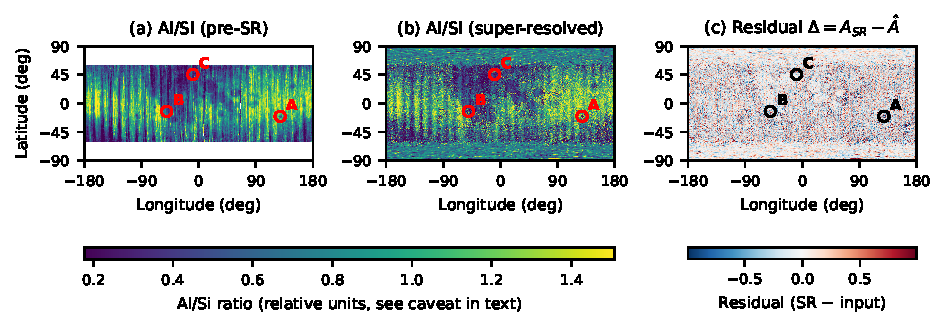
\includegraphics[width=\textwidth]{../outputs/figures/final/fig3_sr_sidebyside.pdf}
  \caption{Al/Si ratio map before (a) and after (b) cross-modal guided
    super-resolution ($\alpha=1.0$, full detail injection,
    \cref{tab:ablation}), shown on the $|\phi|<60^{\circ}$ analysis band
    at the native $1080\times540$ ($\sim0.33^{\circ}$) resolution, plus
    (c) the residual $\Delta = \mathbf{A}_{\mathrm{SR}} - \hat{\mathbf{A}}$
    (\cref{eq:residual}, diverging scale, white = no change). Panel (c)
    shows the SR stage adds structured, crater- and ejecta-shaped detail
    rather than uniform noise, i.e.\ spatially coherent with real optical
    features rather than a fusion artefact. Circles mark the three pixels
    with the largest $|\Delta|$, identified programmatically. Colorbar
    units in (a)/(b) are the relative Al/Si ratio
    (\cref{sec:units_caveat}), not wt\%.}
  \label{fig:sr_sidebyside}
\end{figure*}

The blending-weight ablation (\cref{tab:ablation}) varies
$\alpha \in \{0.1, 0.3, 0.5, 0.7, 1.0\}$ for Al/Si. RMS residual grows and
SSIM-vs.-nearest-neighbour-input falls monotonically with $\alpha$ --
expected, since SSIM here measures similarity to the noisy, blocky
\emph{input} map, and guided SR's purpose is to move away from that
baseline toward genuine sub-footprint detail borrowed from the optical
guide; maximising SSIM against a noisy reference would trivially select
the smallest $\alpha$, i.e.\ the least detail injected, not a meaningful
operating point. We instead report $\alpha=1.0$ (full injection,
\cref{eq:rescale,eq:fusion}) as the operating point used throughout,
consistent with standard pansharpening practice, and use the correlation
and regression diagnostics of
\cref{sec:sr_correlation,sec:sr_regression} -- not SSIM-vs.-baseline --
to justify which elements should be super-resolved at all.

\begin{table}[!t]
  \centering
  \caption{Ablation over the blending weight $\alpha$ (\cref{eq:fusion})
    for Al/Si. Poly.\ degree, $R^2$, MAE are from the fixed regression
    $F_{d^*}$ (\cref{eq:poly_regression}), independent of $\alpha$; RMS
    residual and SSIM/PSNR (measured against the noisy nearest-neighbour
    \emph{input}, not ground truth) are reported for transparency -- their
    monotonic trend reflects more injected detail, not degrading fit
    quality (see text).}
  \label{tab:ablation}
  \begin{tabular}{cccccc}
    \toprule
    $\alpha$ & $R^2$ & MAE & RMS residual & SSIM & PSNR (dB) \\
    \midrule
    0.1 & 0.1872 & 0.2573 & 0.1586 & 0.2740 & 13.63 \\
    0.3 & 0.1872 & 0.2573 & 0.1899 & 0.2066 & 13.44 \\
    0.5 & 0.1872 & 0.2573 & 0.2424 & 0.1470 & 13.07 \\
    0.7 & 0.1872 & 0.2573 & 0.3052 & 0.1068 & 12.57 \\
    1.0 & 0.1872 & 0.2573 & 0.4085 & 0.0702 & 11.65 \\
    \bottomrule
  \end{tabular}
\end{table}

\subsection{Validation}\label{sec:validation}

Fitted concentrations were compared, in ratio space (element/Si, per
\cref{sec:units_caveat}), against Apollo and Luna landing-site
geochemistry \cite{LSC}. Footprints within $5^{\circ}$ of each of nine
reference sites (Apollo~11/12/14/15/16/17 and Luna~16/20/24) were matched;
with the expanded dataset \emph{all nine} sites now have between 877 and
1{,}323 matching footprints each, a large improvement over the earlier
subset where several sites had few or none. Because a small number of fits
have near-zero $C_{\mathrm{Si}}$ and produce non-physical ratio outliers,
the median (not mean) ratio per site was used.
\Cref{tab:validation} reports the summary statistics for all five
elements; \cref{fig:validation_scatter} shows the scatter for aluminium,
the only element with a real diagonal trend (the other four scatter
near-flat, fully summarised by their $r$/RMSE/bias in \cref{tab:validation}
without adding visual information).

\begin{figure}[!t]
  \centering
  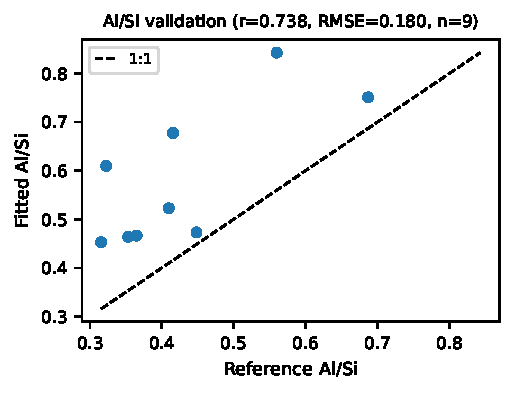
\includegraphics[width=\linewidth]{../outputs/figures/final/fig4_validation_scatter.pdf}
  \caption{Fitted vs.\ reference Al/Si ratio at nine matched Apollo/Luna
    landing sites. Dashed line is the 1:1 reference.}
  \label{fig:validation_scatter}
\end{figure}

\begin{table}[!t]
  \centering
  \caption{Validation against Apollo/Luna landing-site geochemistry,
    ratio-to-Si space, $n=9$ matched sites.}
  \label{tab:validation}
  \begin{tabular}{lccc}
    \toprule
    \textbf{Element} & \textbf{Pearson $r$} & \textbf{RMSE} & \textbf{Bias} \\
    \midrule
    Al & $+0.738$ & 0.180 & $+0.154$ \\
    Ca & $+0.263$ & 0.427 & $-0.422$ \\
    Ti & $-0.117$ & 0.101 & $-0.076$ \\
    Mg & $+0.006$ & 1.782 & $+1.776$ \\
    Fe & $-0.002$ & 0.499 & $-0.467$ \\
    \bottomrule
  \end{tabular}
\end{table}

Aluminium is by far the best-validated element ($r=+0.738$, RMSE 0.18),
independently confirming its selection as the headline element for
super-resolution (\cref{sec:results_sr}): the fitted Al/Si ratio tracks
true landing-site geochemistry across all nine sites, with a consistent
positive bias ($+0.154$, \cref{tab:validation}) that a one-point linear
calibration could plausibly remove. Calcium is weakly positive
($r=+0.263$); Fe, Mg, and Ti show essentially no ratio-space correlation
with ground truth, reflecting both their smaller dynamic range across the
sampled sites and the uncalibrated, relative nature of the fitted
concentrations (\cref{sec:units_caveat}). That the same element --
aluminium -- emerges as both the strongest optical correlator and the
best ground-truth match is the paper's principal evidence that the
pipeline recovers a real compositional signal, not merely an internally
consistent one.

\paragraph{Held-out check of the super-resolved product.}\label{sec:sr_heldout}
\Cref{tab:validation} validates the pre-SR ratio, not
$\mathbf{A}_{\mathrm{SR}}$ itself; since no Apollo/Luna data enters the
fusion (\cref{sec:sr_fusion}), sampling both $\mathbf{A}_{\mathrm{SR}}$
and $\hat{\mathbf{A}}$ at the same nine sites is a direct, leakage-free
check of whether SR moves the estimate toward or away from truth. It is
mixed: $r$ falls slightly ($+0.750\to+0.700$) while RMSE and bias both
improve modestly ($0.233\to0.198$; $+0.216\to+0.177$) -- with $n=9$,
neither change is decisive, and both are consistent with a fusion that
redistributes existing map values around a fixed low-pass mean
(\cref{eq:smooth}) rather than adding new ground-truth information.

\section{Discussion}\label{sec:discussion}

Aluminium emerges as the element with the clearest, physically-signed
link between optical brightness and fitted elemental abundance, and
independently as the best-validated element against Apollo/Luna ground
truth ($r=+0.738$), aligning with the anorthosite-highland reasoning
that originally motivated it as the expected headline element. It was
recovered only at scale: on the earlier ten-month subset the Al
correlation was weak and mis-signed, but near-global coverage, the
element/Si \emph{ratio} (which cancels the per-spectrum scale factor),
and the $|\phi|<60^{\circ}$ band (removing the polar grazing-geometry
artefact) reversed that picture. Once corrected, the two clearest
optical tracers behave as lunar geology predicts: highland-forming Al/Si
is the most robust positive correlate ($\rho=+0.43$) and mafic Mg/Si the
most robust negative correlate ($\rho=-0.39$, \cref{tab:correlation}) --
moderate correlations in absolute terms, but correctly and consistently
signed. The other element ratios correlate only weakly with albedo,
which is expected -- albedo is a partial proxy for composition, and each
element's ratio
couples to it to a different degree.

Magnesium illustrates the limits of that proxy: Mg/Si has the
second-largest optical correlation ($\rho=-0.39$) but essentially no
agreement with Apollo/Luna ground truth in ratio space
($r=+0.006$, \cref{tab:validation}), worth reconciling rather than
leaving juxtaposed. We read the optical correlation as tracking the
regional mare/highland albedo contrast -- to which Mg/Si is only one
contributor alongside iron content and weathering maturity -- rather
than element-specific composition at a landing site's point scale; Mg's
soft K$\alpha$ line (1.25\,keV) and the sites' clustering on nearside
maria/highlands are plausible additional factors. Mg/Si is therefore
evidence of a real regional optical-albedo association but not of
validated compositional recovery; only Al carries both forms of
evidence, which is why it alone anchors the headline claims.

Three limitations should be noted. First, the fusion
(\cref{sec:sr_fusion}) injects detail directly from the optical guide,
so injected texture is only as meaningful as the underlying correlation
is strong -- reasonable for Al/Si and Mg/Si ($|\rho|\approx0.4$) but not
the weakly-correlated elements (\cref{tab:correlation}), which is why we
restrict the headline result to Al; a learned, cross-validated fusion
model may better judge \emph{how much} detail to trust per-pixel.
Second, no solar-flux normalisation was applied: fitted concentrations
are scale factors relative to each spectrum's own fit, and the 24
months span a wide range of solar-cycle conditions \cite{Hathaway2015}
without day-to-day correction for incident solar X-ray intensity -- a
plausible residual noise source. Third, \cref{eq:secondary} absorbs the
Sherman formulation's geometry-dependent terms ($\psi$, $\phi$) into $s$
and $\beta_{j,m}$ rather than modelling incidence/emergence angles
explicitly -- standard for a first-pass FP model, but it means absolute
intensities are not directly comparable across very different viewing
geometries.

Future work should prioritise: (i) solar-flux cross-calibration (e.g.\
via the XSM aboard Chandrayaan-2); (ii) a learned replacement for the
polynomial regression of \cref{sec:sr_regression}; (iii) a cross-validated
one-point Al bias calibration (\cref{sec:validation}); and (iv) extending
raw-data coverage toward full completeness.

\section{Conclusion}\label{sec:conclusion}

This paper presented a complete pipeline for lunar elemental abundance
mapping from Chandrayaan-2 CLASS XRF data: a fundamental-parameter
forward model with primary and secondary fluorescence
(\cref{sec:fp_model}), Trust-Region-Reflective spectral fitting
(\cref{sec:fitting}), element/Si ratio spatial mapping
(\cref{sec:mapping}), and a cross-modal optical-guided super-resolution
scheme (\cref{sec:superres}). The pipeline was run end-to-end on
855{,}190 real, newly fitted CLASS spectra drawn from 24 months of raw
data spanning December 2020 to May 2026 (1{,}056{,}619 dayside spectra
before quality filtering), achieving \textbf{99.0\% global map coverage}
at $1^{\circ}$ resolution -- near-complete sampling of the lunar surface.
Aluminium was identified as the element with the clearest, physically-signed
optical--compositional correlation ($\rho=+0.43$ for Al/Si on the reliable
$|\phi|<60^{\circ}$ band, positive as expected for the anorthositic
highlands) and was used as the headline element for the super-resolution
demonstration in \cref{fig:sr_sidebyside}. The same element is
independently the best-validated against Apollo and Luna landing-site
geochemistry (\cref{sec:validation}), with the fitted Al/Si ratio tracking
ground truth at $r=+0.738$ across all nine sites -- strong evidence that
the pipeline recovers a real, geochemically meaningful signal. The
principal limitations --
lack of solar-flux normalisation, a hand-crafted rather than learned
super-resolution model, and concentrations reported in relative rather
than calibrated wt\% units -- are identified explicitly in
\cref{sec:discussion} as the clearest next steps for this line of work.

\section*{Data Availability Statement}
The raw CLASS Level-1 XRF data used in this study are publicly available
via the PRADAN portal (ISSDC/ISRO). The processing pipeline, fitting
code, and analysis scripts are openly available at a GitHub repository,
archived with a permanent DOI via Zenodo: \url{https://github.com/GeeteshPaidi/SomaDhatuNirupana}, \url{https://doi.org/10.5281/zenodo.21993207}. The full-resolution
processed abundance maps for all fitted elements (beyond the Al headline
result presented in the main text) are available as Supplementary
Material.

\section*{Acknowledgements}
The authors thank ISRO and the Indian Space Science Data Centre (ISSDC)
for providing public access to Chandrayaan-2 CLASS data via the PRADAN
portal.

\begin{thebibliography}{21}

\bibitem{Jenkins1999}
R.~Jenkins.
\newblock \emph{X-Ray Fluorescence Spectrometry}.
\newblock John Wiley \& Sons, New York, 2nd edition, 1999.
\newblock \doi{10.1002/9781118521014}.

\bibitem{Beckhoff2006}
B.~Beckhoff, B.~Kanngie{\ss}er, N.~Langhoff, R.~Wedell, and H.~Wolff.
\newblock \emph{Handbook of Practical X-Ray Fluorescence Analysis}.
\newblock Springer-Verlag, Berlin, 2006.
\newblock \doi{10.1007/978-3-540-36722-2}.

\bibitem{Narendranath2020}
S.~Narendranath, P.~S.~Athiray, P.~Sreekumar, et~al.
\newblock Chandrayaan-2 {L}arge {A}rea {S}oft {X}-ray {S}pectrometer
  ({CLASS}): {I}n-flight performance and first results.
\newblock \emph{Current Science}, 118(2):204--209, 2020.

\bibitem{Lawrence1998}
D.~J.~Lawrence, W.~C.~Feldman, B.~L.~Barraclough, A.~B.~Binder,
  R.~C.~Elphic, S.~Maurice, and D.~R.~Thomsen.
\newblock Global elemental maps of the {M}oon: {T}he {L}unar {P}rospector
  gamma-ray spectrometer.
\newblock \emph{Science}, 281(5382):1484--1489, 1998.
\newblock \doi{10.1126/science.281.5382.1484}.

\bibitem{Kodikara2020}
G.~R.~Kodikara and L.~J.~McHenry.
\newblock Machine learning approaches for classifying lunar soils.
\newblock \emph{Icarus}, 345:113719, 2020.

\bibitem{Wu2024}
S.~Wu, J.~Chen, C.~Xue, Y.~Pan, and C.~Zhang.
\newblock Global inversion of lunar surface oxides by adding
  {C}hang'{E}-5 samples.
\newblock \emph{Remote Sensing}, 16(10):1812, 2024.
\newblock \doi{10.3390/rs16101812}.

\bibitem{Wen2024}
S.~Wen, Y.~Wang, Q.~Gong, J.~Liu, X.~Kang, H.~Liu, R.~Chen, K.~Zhu, and
  S.~Zhang.
\newblock A new robust lunar landing selection method using the {B}ayesian
  optimization of extreme gradient boosting model ({BO}-{XGB}oost).
\newblock \emph{Remote Sensing}, 16(19):3632, 2024.
\newblock \doi{10.3390/rs16193632}.

\bibitem{Yang2023}
C.~Yang, X.~Zhang, L.~Bruzzone, B.~Liu, D.~Liu, X.~Ren, J.~A.~Benediktsson,
  Y.~Liang, B.~Yang, M.~Yin, H.~Zhao, R.~Guan, C.~Li, and Z.~Ouyang.
\newblock Comprehensive mapping of lunar surface chemistry by adding
  {C}hang'{E}-5 samples with deep learning.
\newblock \emph{Nature Communications}, 14:7554, 2023.
\newblock \doi{10.1038/s41467-023-43358-0}.

\bibitem{Mallat2009}
S.~Mallat.
\newblock \emph{A Wavelet Tour of Signal Processing: The Sparse Way}.
\newblock Academic Press, 3rd edition, 2009.

\bibitem{Savitzky1964}
A.~Savitzky and M.~J.~E.~Golay.
\newblock Smoothing and differentiation of data by simplified least
  squares procedures.
\newblock \emph{Analytical Chemistry}, 36(8):1627--1639, 1964.

\bibitem{Sherman1955}
J.~Sherman.
\newblock The theoretical derivation of fluorescent {X}-ray intensities
  from mixtures.
\newblock \emph{Spectrochimica Acta}, 7:283--306, 1955.
\newblock \doi{10.1016/0371-1951(55)80041-0}.

\bibitem{Shiraiwa1966}
T.~Shiraiwa and N.~Fujino.
\newblock Theoretical calculation of fluorescent {X}-ray intensities in
  fluorescent {X}-ray spectrochemical analysis.
\newblock \emph{Japanese Journal of Applied Physics}, 5(10):886--899, 1966.
\newblock \doi{10.1143/JJAP.5.886}.

\bibitem{Criss1968}
J.~W.~Criss and L.~S.~Birks.
\newblock Calculation methods for fluorescent {X}-ray spectrometry:
  Empirical coefficients vs.\ fundamental parameters.
\newblock \emph{Analytical Chemistry}, 40(7):1080--1086, 1968.
\newblock \doi{10.1021/ac60263a023}.

\bibitem{Schoonjans2011}
T.~Schoonjans, A.~Brunetti, B.~Golosio, M.~{Sanchez del Rio},
  V.~A.~Sol{\'e}, C.~Ferrero, and L.~Vincze.
\newblock The \texttt{xraylib} library for {X}-ray--matter interactions.
  {R}ecent developments.
\newblock \emph{Spectrochimica Acta Part B: Atomic Spectroscopy},
  66(11--12):776--784, 2011.
\newblock \doi{10.1016/j.sab.2011.09.011}.

\bibitem{Branch1999}
M.~A.~Branch, T.~F.~Coleman, and Y.~Li.
\newblock A subspace, interior, and conjugate gradient method for
  large-scale bound-constrained minimization problems.
\newblock \emph{SIAM Journal on Scientific Computing}, 21(1):1--23, 1999.
\newblock \doi{10.1137/S1064827595289108}.

\bibitem{Ham2018}
B.~Ham, M.~Cho, and J.~Ponce.
\newblock Robust guided image filtering using nonconvex potentials.
\newblock \emph{IEEE Transactions on Pattern Analysis and Machine
  Intelligence}, 40(1):192--207, 2018.
\newblock \doi{10.1109/TPAMI.2017.2669034}.

\bibitem{Vivone2015}
G.~Vivone, L.~Alparone, J.~Chanussot, et~al.
\newblock A critical comparison among pansharpening algorithms.
\newblock \emph{IEEE Transactions on Geoscience and Remote Sensing},
  53(5):2565--2586, 2015.

\bibitem{Lucey2000}
P.~G.~Lucey, D.~T.~Blewett, G.~J.~Taylor, and B.~R.~Hawke.
\newblock Imaging of lunar surface maturity.
\newblock \emph{Journal of Geophysical Research: Planets},
  105(E8):20377--20386, 2000.
\newblock \doi{10.1029/1999JE001110}.

\bibitem{Smith1997}
S.~W.~Smith.
\newblock \emph{The Scientist and Engineer's Guide to Digital Signal
  Processing}.
\newblock California Technical Publishing, 1997.

\bibitem{LSC}
C.~Meyer.
\newblock \emph{Lunar Sample Compendium}.
\newblock NASA Johnson Space Center, Houston, TX, 2012.
\newblock \url{https://curator.jsc.nasa.gov/lunar/compendium.cfm}.

\bibitem{Hathaway2015}
D.~H.~Hathaway.
\newblock The solar cycle.
\newblock \emph{Living Reviews in Solar Physics}, 12:4, 2015.
\newblock \doi{10.1007/lrsp-2015-4}.

\end{thebibliography}

\end{document}
